\chapter{Evaluation}

\chapterintro{
  This chapter contains results and discussions on the evaluation of tests run on the proposed solution.
}

\section{Introduction}
We carried out a number of tests which aim to prove the solution be better than currently available, especially in terms of:
\begin{enumerate}
  \item deployment cost
  \item cost of providing given Quality-of-Service
  \item deployment time
\end{enumerate}

\subsection*{Hardware and virtual machines configuration}
Many of the carried out tests were run on the same hardware and/or used the same virtual machines so for clarity of presentation their parameters are presented not in a description of every test, but here in table \ref{tbl:test-deployment-time-common-hardware-configuration}.

\begin{table}
  \centering
  \begin{tabular}{ | l | l | l | l | }
    \hline                        
    Name & CPU & RAM & HD \\
    \hline
    (device) Desktop        & Intel(R) Core(TM) i5-2500 CPU @ 3.30GHz & 8GB & 1TB \\
    (device) Node1        & AMD Athlon\texttrademark 64 X2 Dual Core, 2000MHz & 3GB & 160GB \\
    (device) Node3        & AMD Sempron(tm) Processor 3000+ & 2.5GB & 160GB \\
    (device) Node4        & AMD Duron(tm) Processor 1GHz& 2.5GB & 60GB \\
    (virtual machine) Frontend\{1,2\}  & 1 CPU & 512MB & 10GB \\
    \hline  
  \end{tabular}
  \caption{Configuration of hardware/virtual machines used during tests}
  \label{tbl:test-deployment-time-common-hardware-configuration}
\end{table}

\section{Cost of service deployment}
\subsection*{Description}
The aim of this test case is to test the primary use case of the proposed solution -- deployment of a service with the emphasis of client's \textbf{cost}. It should show that the platform chooses the best mapping between the stacks and cloud providers so that the client's pays the \textbf{lowest} possible price.

\subsection*{Preconditions}
Service specification (\ref{lst:service-spec-test-cost}) forms an input to the application. Its elements are different software stacks that are parts of the whole service. Each cloud provider has its own price for a given software stack which is shown in table \ref{tbl:test-service-deployment-cost}. Diagram \ref{eval:deployment-cost-physical-nodes} illustrates the simplified environment setup.

\begin{table}
  \centering
  \begin{tabular}{ | c | c | c | c | }
    \hline                        
    & CP-1 & CP-2 & CP-3 \\
    \hline
    java      & 150 & 120 & 180 \\
    ruby      & 220 & 290 & 250 \\
    postgres  & 320 & 240 & 290 \\
    python    & 200 & 260 & 180 \\
    amqp      & 330 & 390 & 285 \\
    \hline  
  \end{tabular}
  \caption{Price for a stack in the given cloud provider}
  \label{tbl:test-service-deployment-cost}
\end{table}

\begin{figure}[!ht]
  \begin{center}
    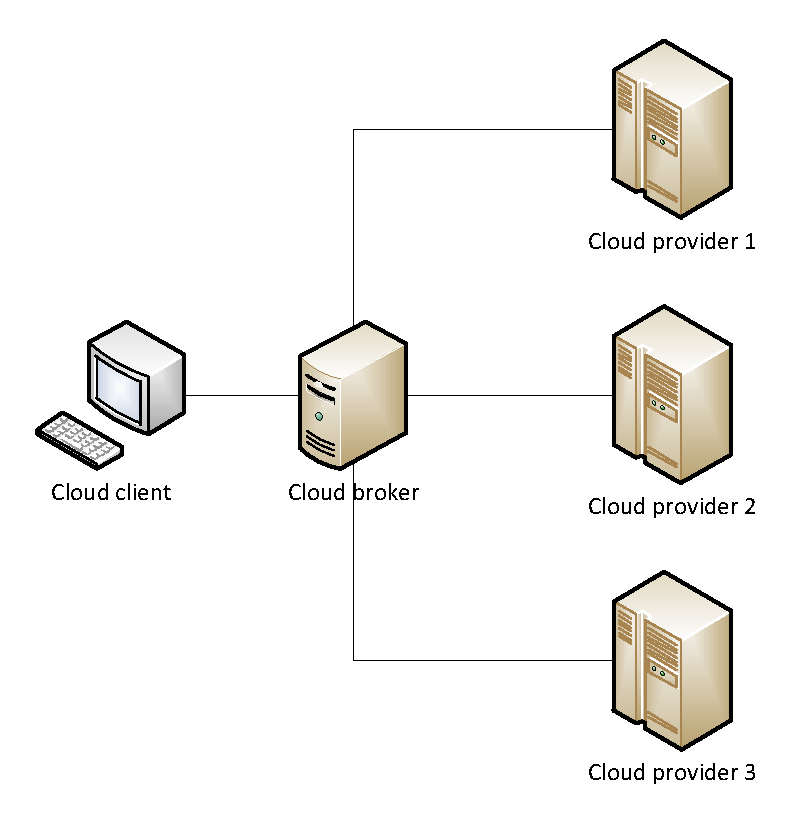
\includegraphics[width=0.6\textwidth]{chapter-7/deployment-cost-physical-nodes}
  \end{center}
  \caption{Deployment cost: environment configuration}
  \label{eval:deployment-cost-physical-nodes}
\end{figure}


\subsection*{Results}
Table \ref{tbl:test-service-deployment-cost-mapping} shows obtained mapping between stacks and cloud providers. Taking into account this result, figure \ref{ch7:service-deployment-cost} shows comparison of cost the client would have to pay with and without such a mapping.

\begin{table}
  \centering
  \begin{tabular}{ | c | c | c | c | }
    \hline                        
    & CP-1 & CP-2 & CP-3 \\
    \hline
    java      & & x & \\
    ruby      & x & & \\
    postgres  & & x & \\
    python    & & & x \\
    amqp      & & & x \\
    \hline  
  \end{tabular}
  \caption{Chosen cloud providers for the given stack}
  \label{tbl:test-service-deployment-cost-mapping}
\end{table}

\begin{figure}[!ht]
  \begin{center}
    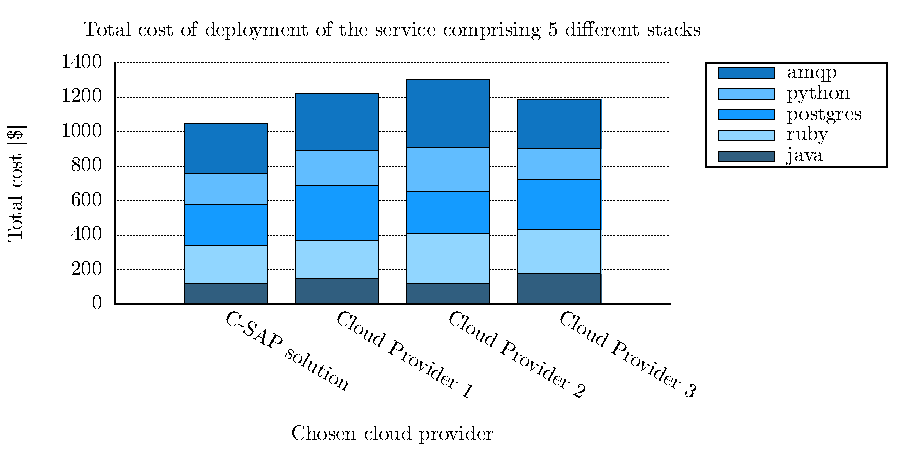
\includegraphics{chapter-7/case-study-service-deployment-reduced-client-costs}
  \end{center}
  \caption{Comparison of the deployment cost when the service is deployed only on a selected cloud provider or a combination of cloud providers selected by Cloud-SAP}
  \label{ch7:service-deployment-cost}
\end{figure}

\subsection*{Conclusion}
Obtained results clearly show that our proof-of-concept product met expectations of this test case as the client was offered the cheapest deployment scheme among various cloud providers for a given software stack.
The mapping mechanism is simple yet considerably powerful -- in this simple scenario the savings were significant since they constituted nearly 20 percent of the price offered by \emph{Cloud Provider 2}. This shows that implementing similar solutions in the real world could be of great benefit to cloud consumers.

\section{Auto-scaling -- single-provider based}
\subsection*{Description}
\begin{asparaenum}
\item[\textbf{Motivation}]The aim of this test-case is to show that introducing a multi-layered auto-scaling platform is of a great benefit in terms of cost and resource usage for cloud consumers and cloud providers respectively. What is more, this test should prove that once there are many levels on which scaling operations can be performed, there are significant reduction in costs paid by consumers.
We want to prove it by comparing our proof-of-concept product to \emph{Carina} \cite{Carina}. \emph{Carina} embraces a whole range of various scaling policies for users' environments (environment, in this context, means an application with all its software dependencies that are to be deployed on the cloud), but there is only one way in which they are executed -- by managing the number of virtual machines (i.e. horizontal scaling). Quite on the contrary, \emph{Cloud-SAP} has mechanisms that allow to scale the environment vertically in the first place and if that turns out to be not sufficient, horizontally. This test shows the influence of lack/presence of this feature on price and resource consumption.
\item[\textbf{Scenario}] The test scenario involves
  \begin{inparaenum}[a)]
    \item deployment of a sample environment on the cloud,
    \item substitute the real module responsible for collecting CPU usage date for a mock one,
    \item monitoring the scaling actions performed by each solution,
    \item evaluation of the cost the client has to pay for the service.
  \end{inparaenum}
  Deployment of a service is done in a product-specific manner (up to the point where the vm deployment request is passed to OpenNebula). Mocking the CPU usage was possible by replacing the part in \emph{InformationManager} responsible the collecting CPU data in a host for a request to a web service which generated a time-based mocked-values. Choosing the appropriate function is another issue and is discussed in the next paragraph.
\end{asparaenum}

\subsubsection*{CPU usage function}
We wanted to ensure that both solutions, \emph{Carina} and \emph{Cloud-SAP}, collected the same data regarding the CPU usage for the given time. What is more, the curve should resemble CPU usage in the real business scenarios as much as possible. Thus, we took into account the following factors:
\begin{itemize}
  \item every peak in CPU usage should be followed by a gradual descent as each solution performs scaling actions,
  \item (boundary conditions) CPU usage should be between 0 and 100 and, additionally, should exceed the previously set scaling threshold value of each solutions so that it would trigger the scaling policies evaluation
  \item once the scaling operations have completed, CPU usage should be constant at a rate which would not introduce any changes in the environment settings (such as the number of virtual machines and parameters of any virtual machine)
\end{itemize}
This resulted in the function whose formula is in \eqref{eq:cpu-mock-usage} and plot in figure \ref{eval:auto-scaling-1cp-cpu-usage-function}.
\begin{eqnarray}
  %f(x) = (1751 *x)/132+(3 *x**2)/8-(31* x**3)/264
  %x <= 11.583 ? f(x) : ( x <= 21.441 ?  f(x - 10) : 25 )
  f(x) &=& -\frac{31}{264}x^3+\frac{3}{8}x^2+\frac{1751}{132}x \nonumber \\
  CPU\_usage(t) &=& \left\{
  \begin{array}{l l l}
    f(t) & \quad 0 & \le t < 11.583 \\
    f(t-10) & \quad 11.583 & \le t < 21.441 \\
    25 & \quad 21.441 & \le  t \\
\end{array} \right.
\label{eq:cpu-mock-usage}
\end{eqnarray}

\begin{figure}[!ht]
  \begin{center}
    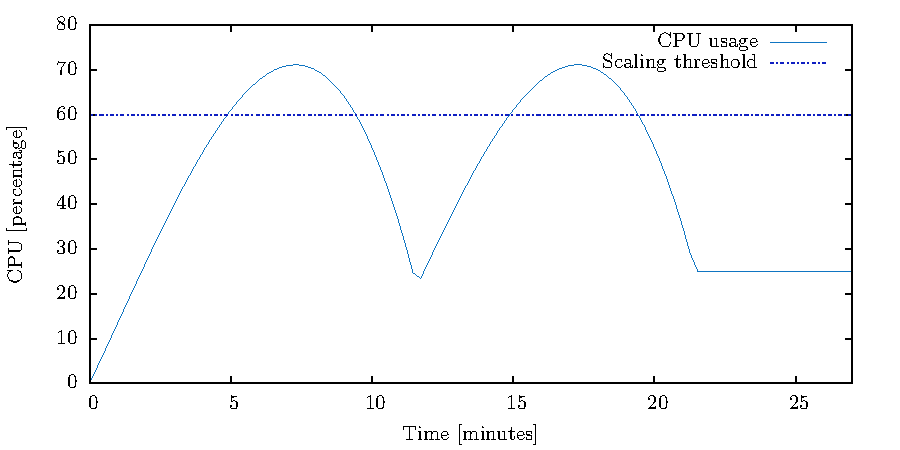
\includegraphics{chapter-7/cpu-usage-mock}
  \end{center}
  \caption{Auto-scaling - single-provider based: CPU usage function}
  \label{eval:auto-scaling-1cp-cpu-usage-function}
\end{figure}

Because \emph{Carina} is capable of only horizontal scaling and \emph{Cloud-SAP} of both horizontal and vertical, one can question whether the descent in CPU usage can be actually the same in both cases. To answer this question we want to look into the description of the virtual machines comprising the deployed environment. It states that each VM can use up to 30\% power of the CPU of a host. Thus, we can be fairly sure that adding another virtual machine that uses 0.3 CPU capacity of its host is equivalent with changing the CPU usage settings of already deployed VM from 30 to 60\%.
\subsection*{Preconditions}
\subsubsection*{Environment specification}
\begin{asparaenum}
  \item[\textbf{Auto-scaling policy specifications}] As it is shown in figure \ref{eval:auto-scaling-1cp-cpu-usage-function}, we set in both products the threshold values of CPU usage that trigger performing auto-scaling actions to 20 and 60 percent. To apply this setting, the auto-scaling part of service specification looks as follows: in Carina the user has to add the parameters of an auto-scaling policy in a hash that describes the environment under key \emph{:elasticy\_policy}. It is possible to specify the minimal and the maximal number of virtual machines that forms the environment and, what is most important, expressions which evaluation results in scaling the application. The part responsible for this is shown in listing \ref{lst:auto-scaling-1cp-carina-service-spec}.\lstinputlisting[caption=Carina service specification used for testing auto-scaling with 1 cloud provider, label=lst:auto-scaling-1cp-carina-service-spec]{auto-scaling-1cp-carina-service-spec} In Cloud-SAP it is a matter of setting appropriate arguments to a specific policy. In this case the policy is \emph{threshold\_model} and values are 20 and 60 for lower and upper bound respectively. The auto-scaling part from service specification is shown in listing \ref{lst:auto-scaling-1cp-cloud-sap-service-spec}. \lstinputlisting[caption=Cloud-SAP service specification used for testing auto-scaling with 1 cloud provider, label=lst:auto-scaling-1cp-cloud-sap-service-spec]{auto-scaling-1cp-cloud-sap-service-spec}
  \item[\textbf{OpenNebulaa/Carina/Cloud-SAP configuration}] Since Carina and Cloud-SAP used two different instances of OpenNebula installed on separate virtual machines, it is essential the configuration be the same on each of them. Listing \ref{lst:auto-scaling-1cp-one-config} shows the most important OpenNebula excerpt from settings file used in this test case -- polling interval specification, which was set to 30 seconds. To ensure that both products can actually use up-to-date data, they should evaluate their policies every 30 seconds or longer. In Carina the user cannot specify this value, because it is hard-coded in source code to 60 seconds. In Cloud-SAP, however, this value was set in a configuration file and was equal to 60 seconds as well as in Carina. \lstinputlisting[caption=OpenNebula configuration excerpt -- information manager, label=lst:auto-scaling-1cp-one-config]{auto-scaling-1cp-one-config}
  \item[\textbf{Deployment diagrams}] Deployment diagrams show the placement of each component in both installations. They are shown in figures \ref{eval:auto-scaling-1cp-carina-deployment-diagram} and \ref{eval:auto-scaling-1cp-cloud-sap-deployment-diagram}.

  \begin{figure}[!ht]
    \begin{center}
      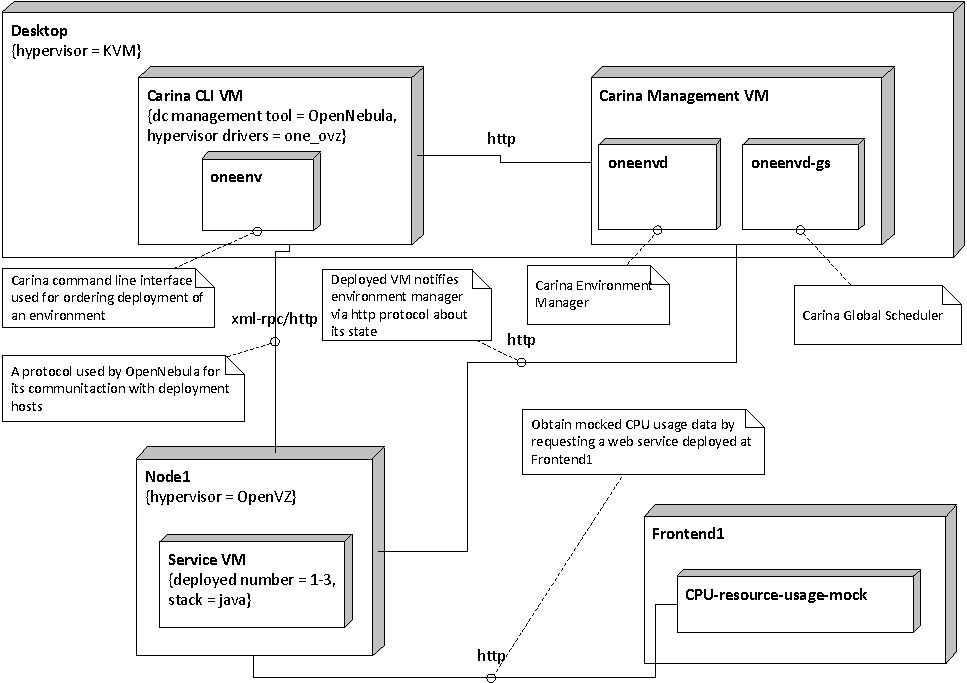
\includegraphics{chapter-7/cpu-usage-carina-deployment-diagram}
    \end{center}
    \caption{Auto-scaling - single-provider based: deployment diagram of Carina}
    \label{eval:auto-scaling-1cp-carina-deployment-diagram}
  \end{figure}

  \begin{figure}[!ht]
    \begin{center}
      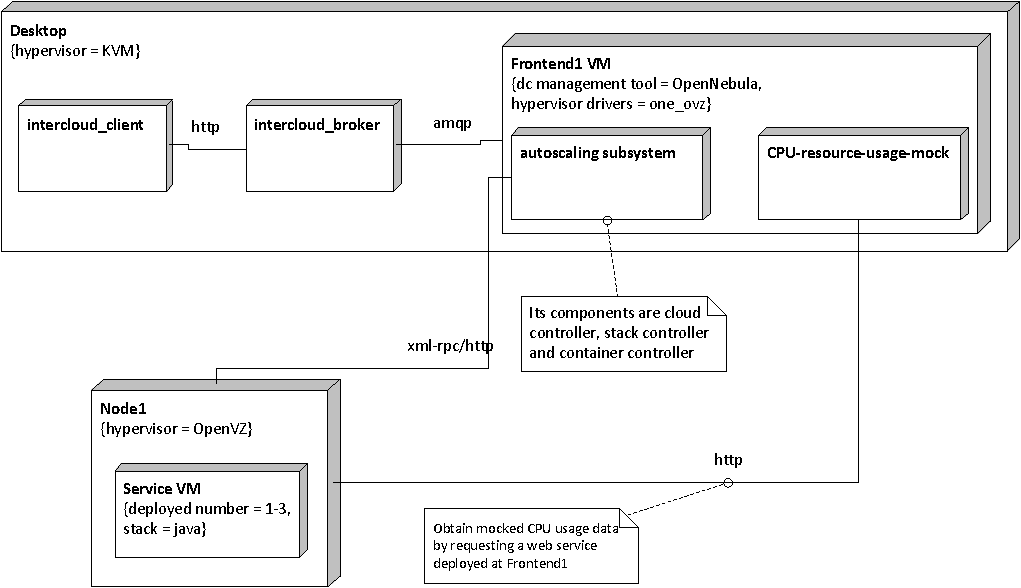
\includegraphics{chapter-7/cpu-usage-cloud-sap-deployment-diagram}
    \end{center}
    \caption{Auto-scaling - single-provider based: deployment diagram of Cloud-SAP}
    \label{eval:auto-scaling-1cp-cloud-sap-deployment-diagram}
  \end{figure}

  \end{asparaenum}

\subsubsection*{Hardware/VM configuration}
All virtual machines were deployed onto \emph{Node1}, which uses \emph{OpenVZ} as a virtualization technology and whose hardware configuration can be found in table \ref{tbl:test-deployment-time-common-hardware-configuration}. \emph{OpenNebula} was installed on a \emph{Frontend1} virtual machine and its configuration is in the same table. \emph{Carina} required the usage of 2 virtual machines which were deployed on \emph{Desktop} with KVM as a hypervisor and whose configuration is in table \ref{tbl:test-auto-scaling-1cp-hardware-configuration}. Diagram \ref{eval:auto-scaling-1cp-physical-nodes} illustrates the physical setup of the test-case.

\begin{table}
  \centering
  \begin{tabular}{ | l | l | l | l | }
    \hline                        
    Name & CPU & RAM & HD \\
    \hline
    (virtual machine) carina-frontend  & 1 CPU & 1GB & 6GB \\
    (virtual machine) carina-management-vm  & 1 CPU & 1GB & 9GB \\
    \hline  
  \end{tabular}
  \caption{Configuration of hardware/virtual machines used during tests}
  \label{tbl:test-auto-scaling-1cp-hardware-configuration}
\end{table}

\begin{figure}[!ht]
  \begin{center}
    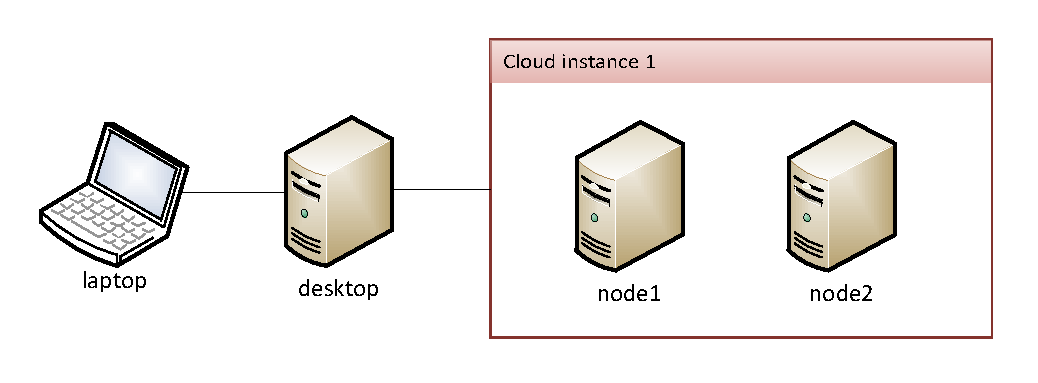
\includegraphics[width=0.8\textwidth]{chapter-7/auto-scaling-1cp-physical-nodes}
  \end{center}
  \caption{Auto-scaling - single-provider based: environment configuration}
  \label{eval:auto-scaling-1cp-physical-nodes}
\end{figure}

\subsection*{Results}
\subsection*{Conclusion}

\section{Auto-scaling -- multiple-provider based}
\subsection*{Description}
\subsection*{Preconditions}
\begin{figure}[!ht]
  \begin{center}
    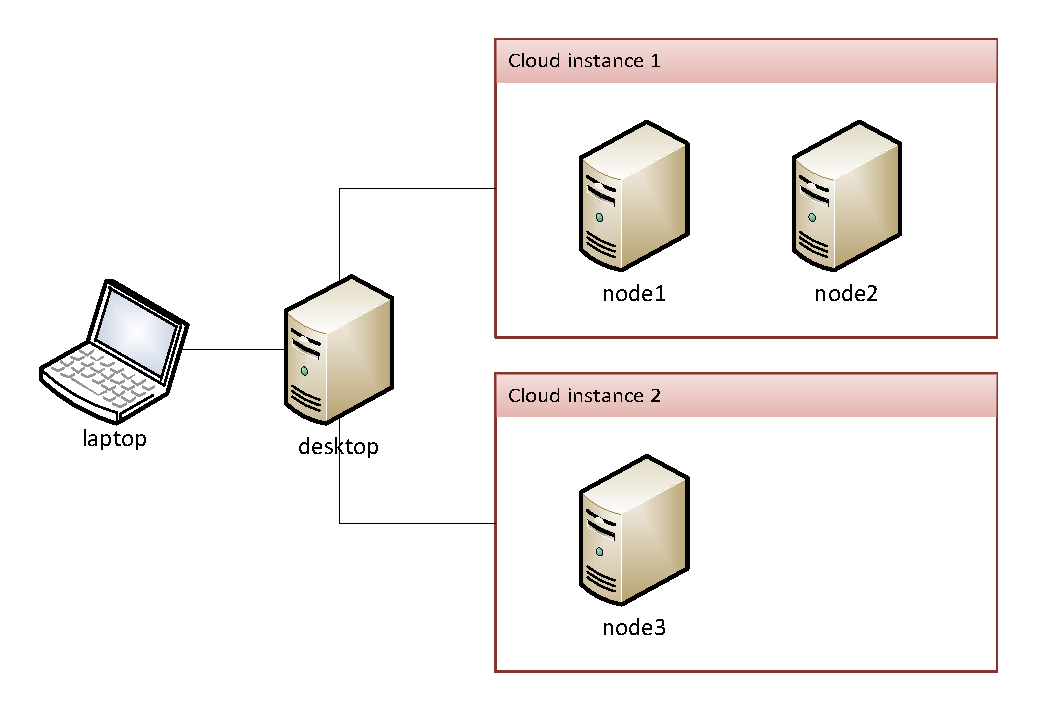
\includegraphics[width=0.8\textwidth]{chapter-7/auto-scaling-2cp-physical-nodes}
  \end{center}
  \caption{Auto-scaling - multiple-provider based: environment configuration}
  \label{eval:auto-scaling-2cp-physical-nodes}
\end{figure}

\subsection*{Results}
\subsection*{Conclusion}

\section{Deployment time -- solution comparison}
\subsection*{Description}
In this test we want to compare our solution to one of those available at the market which use \emph{OpenNebula} as an underlying tool for managing resources of a data center and \emph{OpenVZ} as a hypervisor in terms of \textbf{deployment time}, one of the most important factors of products whose main purpose is to scale applications.
\emph{Carina} \cite{Carina} can be considered a perfect match of a solution for such a comparison and tests are ran against it.

This test involves the steps of
  \begin{inparaenum}[i)]
    \item instantiating one of the tested product, i.e. Cloud-SAP or Carina,
    \item ordering the deployment of a service whose specification is shown in listing \ref{lst:service-spec-test-deployment-time},
    \item measuring the time needed to set up the environment of the service.
  \end{inparaenum}

\subsection*{Preconditions}
It is assumed that \emph{Cloud-SAP} and \emph{Carina} according with \emph{OpenVZ} as an underlying virtualization technology are correctly installed and configured.
Each test case must be run in an isolation so before performing any test all virtual machines present at the deployment node are removed.
\subsubsection{OpenNebula configuration}
To ensure objectivity in tests, OpenNebula was configured in both products in the same way. One of the key factors that could influence the deployment time is the configuration of scheduler. Its parameters are shown in the listing \ref{lst:one-scheduler-config}.
\lstinputlisting[caption=OpenNebula scheduler configuration, label=lst:one-scheduler-config]{deployment-time-test-sched-config}
\subsubsection{Service description}
The service comprises a simple java enterprise application, deployed in a master-slave configuration with one VM set as a load balancer and other nodes that serve as workers, which uses Tomcat as a web container.

The description of a service expressed in Carina format can be found in listing \ref{lst:carina-config}.

- TODO dodać konfigurację każdej z maszyn wirtualnych 

\subsubsection{Hardware configuration}

All virtual machines were deployed on a host named \emph{Node1}, whose configuration can be found in table \ref{tbl:test-deployment-time-common-hardware-configuration}. Diagram presents the physical configuration of nodes.

\begin{figure}[!ht]
  \begin{center}
    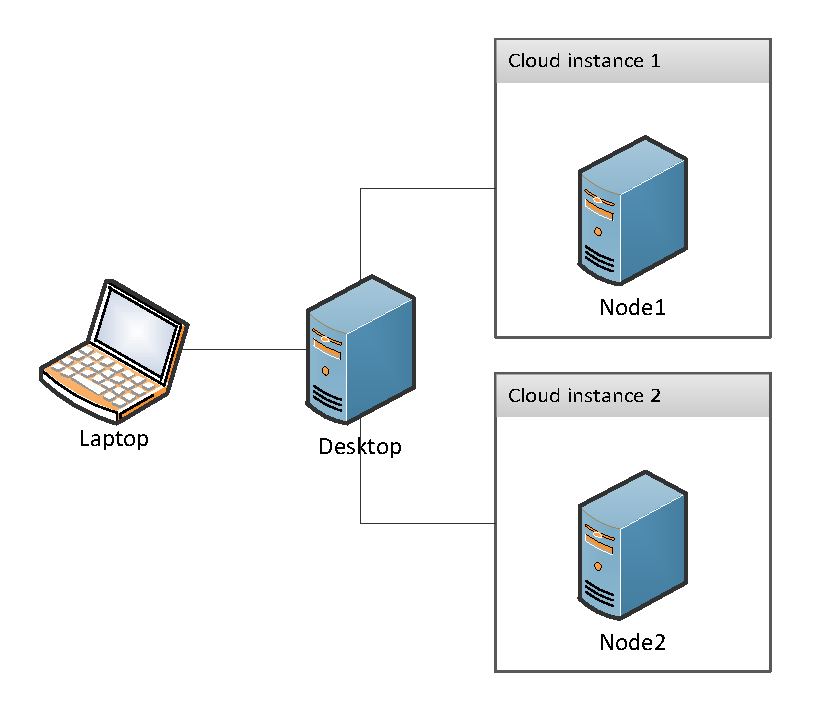
\includegraphics[width=0.6\textwidth]{chapter-7/deployment-time-physical-nodes}
  \end{center}
  \caption{Deployment time - solution comparison: physical environment setup}
  \label{eval:deployment-time-physical-nodes}
\end{figure}

\subsubsection{Environment configuration}
Deployment diagram for \emph{Carina} implementation is shown in figure \ref{ch7:deployment-time-test-deployment-time-carina-deployment-diagram} and for \emph{Cloud-SAP} in figure \ref{ch7:deployment-time-test-cloud-sap-deployment-diagram}.

\begin{figure}[!ht]
  \begin{center}
    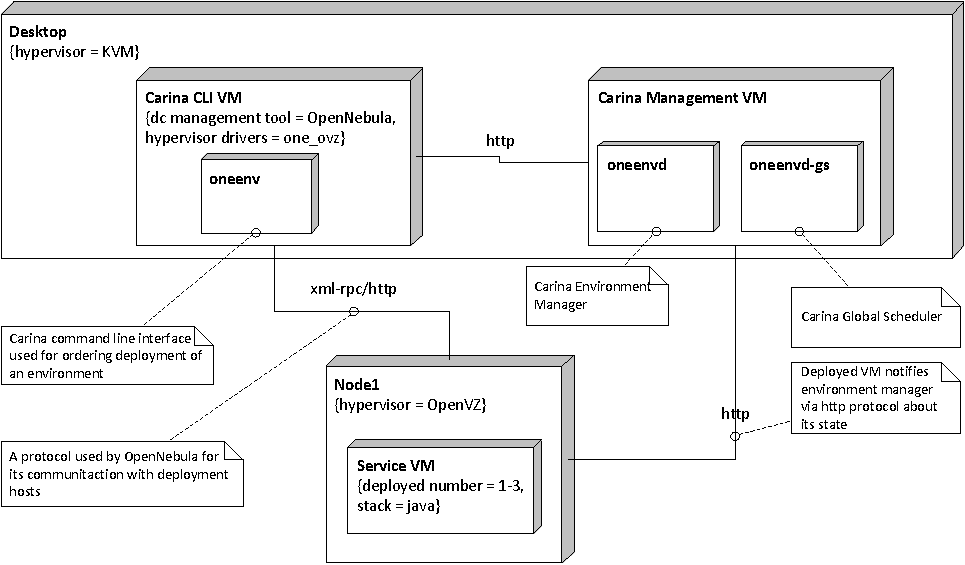
\includegraphics{chapter-7/deployment-time-carina-deployment-diagram}
  \end{center}
  \caption{Deployment diagram of \emph{Carina}}
  \label{ch7:deployment-time-test-deployment-time-carina-deployment-diagram}
\end{figure}

\begin{figure}[!ht]
  \begin{center}
    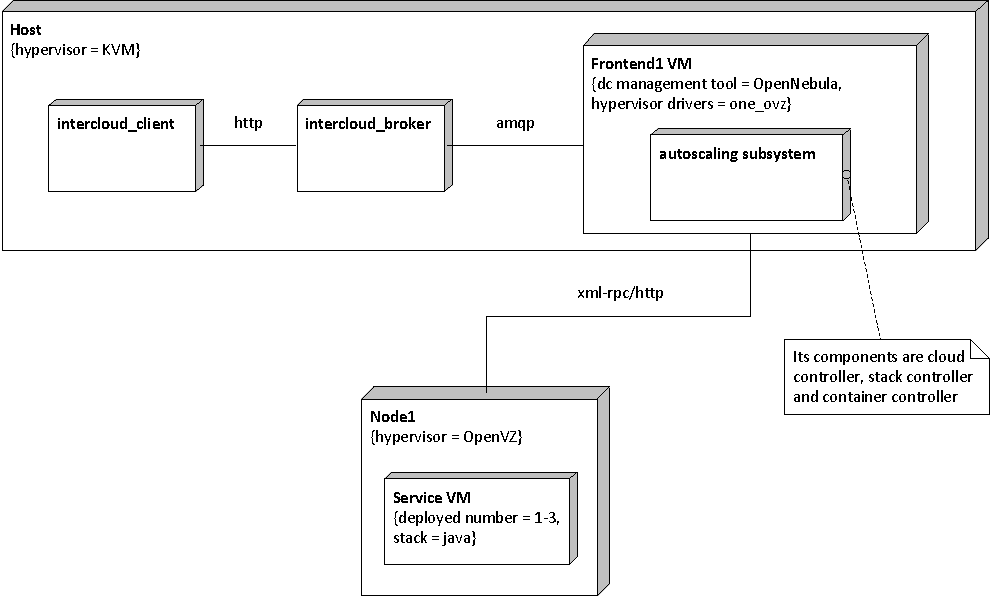
\includegraphics{chapter-7/deployment-time-test-cloud-sap-deployment-diagram}
  \end{center}
  \caption{Deployment diagram of \emph{Cloud-SAP}}
  \label{ch7:deployment-time-test-cloud-sap-deployment-diagram}
\end{figure}

\subsection*{Results}
Obtained results are shown in table \ref{tbl:test-service-deployment-time} and in figure \ref{ch7:deployment-time-test}. For a given number of instances we ordered deploying a service 10 times and the values shown in those figures are an average of these runs.

\begin{table}
  \centering
  \begin{tabular}{ c  c  c }
    \hline
    & \multicolumn{2}{c}{Solution} \\
    \cline{2-3}
    Instance no & Cloud-SAP & Carina \\
    \hline
    2 & 198.0 & 158.7 \\
    3 & 261.72 & 208.1 \\
    4 & 294.38 & 230.6 \\
    \hline
  \end{tabular}
  \caption{Average deployment time for the service with the various number of VMs used for the whole environment}
  \label{tbl:test-service-deployment-time}
\end{table}

\begin{figure}[!ht]
  \begin{center}
    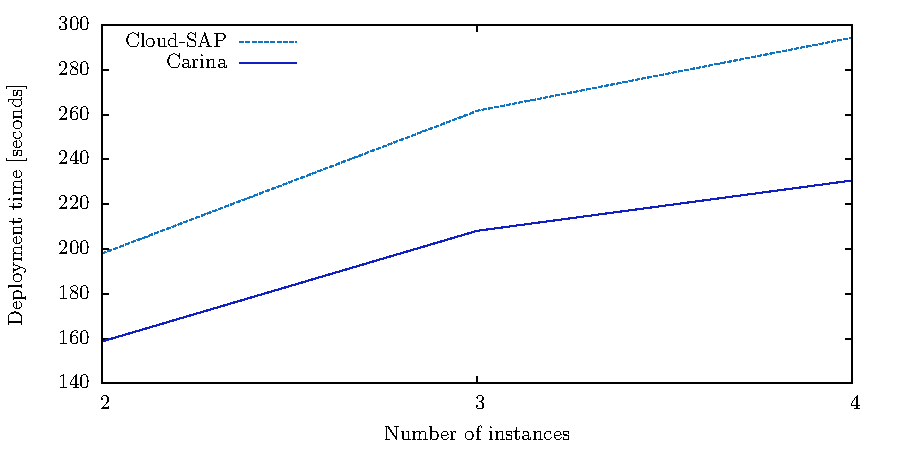
\includegraphics{chapter-7/deployment-time-test}
  \end{center}
  \caption{Average deployment time for two competing products when the variable is the number of instances of VMs}
  \label{ch7:deployment-time-test}
\end{figure}

\subsection*{Conclusion}


\section{Deployment time -- hypervisor comparison}
\subsection*{Description}
\subsection*{Preconditions}
\subsection*{Results}
\subsection*{Conclusion}

